% !TEX root = ../main.tex

\section{Cryptographic Primitives}

\subsection{Discrete Logarithm Assumption:}\label{sec:dlp} The discrete logarithm problem describes, given a triplet $(\mathbb{G}_p, p, g_p)$ and an element $y\in\mathbb{G}_p$, it is infeasible to find an $x$ such that $y=g_p^x$ in polynomial time.

\subsection{Pedersen Commitment:}\label{sec:pedersen} Pedersen's commitment scheme \cite{pedersen} enables $\prv$ to \textit{commit} to a value $x$ without revealing it. Pedersen commitment provides perfectly hiding and computational binding based on the discrete logarithm assumption. Additionally, Pedersen commitments are \textit{additively homomorphic}: given two commitments $C_1$ and $C_2$, the summation of their secrets $x_1$ and $x_2$ is the secret of $C_1+C_2$. We use $\textbf{C}(x)$ to denote a Pedersen commitment to the value $x$. Particularly, we use $\ps$ to denote a Pedersen commitment in secp256k1 and $\pb$ to denote a Pedersen commitment in BLS12-381.

\subsection{$\Sigma-$protocols:}\label{sec:sigma} The $\Sigma-$protocol is a three-move interactive proof system. We define the $\Sigma-$protocol similarly to \cite{damgard10}. \\
\textbf{Definition 1.} \textit{Let $R$ be a binary relation between the statement $x$ and the witness $w$. Given common input $x$ to }$\prv$\textit{ and }$\vrf$\textit{, and private input $(x,w)$ such that $(x,w)\in{R}$ to }$\prv$\textit{, they run the following protocol:}
\begin{enumerate}
    \item $\prv$ \textit{computes a message $m$ from $(x,w)$ and sends $m$.}
    \item $\vrf$ \textit{sends a random challenge $c$.}
    \item $\prv$ \textit{replies with $z$.}
\end{enumerate}
\textit{At the end of the protocol }$\vrf$ \textit{has the data $(x,m,c,z)$}. \textit{He decides to output }\textbf{acc}\textit{ or }\textbf{rej}\textit{; such that}
\begin{itemize}
    \item \textbf{\textit{Completeness}:} \textit{A $\Sigma-$protocol is complete if} $\prv$ \textit{follows the protocol to generate the message $(m,c,z)$,} $\vrf$ \textit{always accepts.}
    \item \textbf{\textit{Special soundness}:} \textit{A $\Sigma-$protocol is special sound if there exists a $\ppt$ extractor $\mathcal{E}$, given any input $x$ and any two accepting $(m,c,z),(m,c^\prime,z^\prime)$ where $c\ne{c^\prime}$, $\mathcal{E}$ can compute $w$ where $(x,w)\in{R}$.}
    \item \textbf{\textit{Honest verifier zero-knowledge}:} \textit{A $\Sigma-$protocol is honest verifier zero-knowledge if there exists a $\ppt$ simulator $\mathcal{S}$, such that the transcript produced by $\mathcal{S}$ is indistinguishable from the messages between }$\prv$\textit{ and }$\vrf$\textit{.}
\end{itemize}
A commonly well-known way to convert a $\Sigma-$protocol into non-interactive is using the Fiat-Shamir transform \cite{fs}. But we still use the standard interactive $\Sigma-$protocol to demonstrate our work for comprehension.

\subsection{OR Proof:}The OR proof allows $\prv$ to convince $\vrf$ that given two inputs $x_1,x_2$, he knows $w$ such that $(x_1,w)\in{R_1}$ or $(x_2,w)\in{R_2}$, but $\vrf$ cannot learn which one $\prv$ knows. We use the same definition as \cite{damgard10}. \\
\textbf{Definition 2.} \textit{The OR proof is a $\Sigma-$protocol that given two inputs $x_1,x_2$,} $\prv$ and $\vrf$ \textit{run the following protocol:}
\begin{enumerate}
    \item $\prv$ \textit{computes the message $m_1$ using $(x_1,w)$ as input.} \\
    $\prv$ \textit{randomly generates $c_2$ as the challenge for $x_2$ and runs the simulator $\mathcal{S}(x_2,c_2)$ to produce $(m_2,z_2)$.}
    \item $\prv$ \textit{sends $m_1$ and $m_2$.}
    \item $\vrf$ \textit{sends a master challenge $c$.}
    \item $\prv$ \textit{computes $c_1=c\oplus{c_2}$ and $z_1$ on inputs $(x_1,c_1,m_1,w)$.} \\
    $\prv$ \textit{sends $(c_1,c_2,z_1,z_2)$.}
\end{enumerate}
\textit{At the end of the protocol} $\vrf$ \textit{verifies $c=c_1\oplus{c_2}$ and both $(m_1,c_1,z_2)$ and $(m_2,c_2,z_2)$ are valid to output} \textbf{acc} \textit{or} \textbf{rej}\textit{; such that}
\begin{itemize}
    \item \textit{\textbf{Completeness:} The case of $c_2$ is always accepted by} $\vrf$ \textit{as the definition of a simulator; on the other side, the case of $c_1$ has no difference from the standard $\Sigma-$protocol. Therefore, the OR proof is complete.}
    \item \textit{\textbf{Soundness:} Let} $\prv$ \textit{execute the protocol twice. Two transcripts} 
    \[ (x_1,x_2,c,c_1,c_2,z_1,z_2),(x_1,x_2,c^\prime,c_1^\prime,c_2^\prime,z_1^\prime,z_2^\prime),c\ne{c^\prime} \] 
    \textit{are given. Then an extractor $\mathcal{E}$ can be constructed by combining two pairs of transcripts $(m_1,c_1,z_1),(m_1^\prime,c_1^\prime,z_1^\prime)$ and $(m_2,c_2,z_2),(m_2^\prime,c_2^\prime,z_2^\prime)$ to compute $x_1$ and $x_2$ respectively.}
    \item \textit{\textbf{Honest verifier zero-knowledge}: Given a master challenge $c$, choose $c_1$ or $c_2$ randomly and the other will be determined. Let the simulator run twice: $\mathcal{S}(x_1,c_1),\mathcal{S}(x_2,c_2)$. }
\end{itemize}
We use $x={x_1\orproof{x_2}}$ to denote $x$ is $x_1$ or $x_2$.

\subsection{Polynomial Commitment Scheme:}\label{sec:pcs} A polynomial commitment scheme (PCS) allows $\prv$ to commit to a polynomial to convince $\vrf$ that claimed evaluations are of the committed polynomial \cite{kzg}. We define PCS based on \cite{kzg,plonk,bdfg}. \\
\textbf{Definition 3.} \textit{A polynomial commitment scheme consists of three moves:} \textbf{gen}\textit{,} \textbf{com}\textit{, and} \textbf{open} \textit{such that}
\begin{enumerate}
    \item \textbf{gen}$(d)$ \textit{is an algorithm that given a random number $\tau\in\mathbb{F}$ and a positive integer d, outputs a structured reference string (SRS)} \textbf{srs} \textit{such that} 
    \[ \textbf{srs}=([1]_1,[\tau]_1,\dots,[\tau^{d-1}]_1,[1]_2,[\tau]_2) \]
    \item \textbf{com}(\textit{f}, \textbf{srs}) \textit{outputs a commitment} $\cm$ \textit{to f, where f is a polynomial over $\mathbb{F}$ of degree smaller than d.}
    \item \textbf{open} \textit{is a protocol that} $\prv$ \textit{is given input f}, \textit{and} $\prv$ \textit{and} $\vrf$ are both given
    \begin{itemize}
        \item \textbf{srs}
        \item $\cm$ - \textit{the commitment to $f$}
        \item $a$ - \textit{an evaluation point of $f$}
        \item $b$ - \textit{the claimed evaluation of $f(a)$}
    \end{itemize}
    \textit{They run the protocol as follows:}
    \begin{enumerate}
        \item $\prv$ \textit{reveals the proof $\pi$ for the pair $(a,b)$ where}
        \[ \pi=[\frac{f(x)-b}{x-a}]_1 \]
        \item $\vrf$ \textit{outputs} \textbf{acc} \textit{if and only if}
        \[ e(\cm-[b]_1,[1]_2)=e(\pi,[\tau-a]_2) \]
    \end{enumerate}
\end{enumerate}
\begin{itemize}
    \item \textit{\textbf{Completeness}: It is clear that $\pi$ exists if and only if $f(a)=b$, which means $\vrf$ always accepts the proof if $\prv$ follows the protocol.}
    \item \textit{\textbf{Knowledge soundness in the algebraic group model}: For any algebraic adversary $\mathcal{A}$ in an interactive protocol of PCS, there exists a $\ppt$ extractor $\mathcal{E}$ given access to $\mathcal{A}$'s messages during the protocol, and $\mathcal{A}$ can win the following game with negligible probability:}
    \begin{enumerate}
        \item \textit{Given the inputs that} $\prv$ \textit{can access, $\mathcal{A}$ outputs} $\cm$.
        \item \textit{$\mathcal{E}$ outputs $f\in\mathbb{F}_{<d}[X]$ from $\mathcal{A}$'s output.}
        \item \textit{$\mathcal{A}$ generates $\pi$ and the evaluation $b^\prime$ at the evaluation point $a$.}
        \item \textit{$\mathcal{A}$ wins if}
        \begin{itemize}
            \item $\vrf$ \textit{accepts the proof at the end of the protocol.}
            \item $b^\prime\ne{b}$.
        \end{itemize}
    \end{enumerate}
\end{itemize}
Our work uses PCS with the root of unity. We use $\omega$ to denote the root of unity. We use $[f]_1$ and $\cm_f$ to denote a commitment to $f$ interchangeably.

\subsection{Open KZG with Committed Value}
\label{sec:kzgOpenComm}
By Definition 3, to prove $b$ is the evaluation of $f(a)$, $\prv$ reveals the pair $(a,b)$ to let $\vrf$ validate the proof through pairings. However, this leaks the evaluation at the point $a$. \bootstrap uses the variaint of this opening techinque. Here we describe the new opening scheme. \\
\textbf{openToCommit} \textit{is a protocol that} $\prv$ \textit{is given input $f$ and $b$}. $\prv$ \textit{and} $\vrf$ are both given
\begin{itemize}
    \item \textbf{srs}
    \item $\cm$
        \item $a$ - \textit{an evaluation point of $f$}
\end{itemize}
\textit{They run the protocol as follows:}
\begin{enumerate}
    \item $\prv$ \textit{reveals the proof $\pi$ for the pair $(a,b)$ where}
    \[ \pi=[\frac{f(x)-b}{x-a}]_1 \]
    \item \textit{Instead of sending $(a,b)$ directly, $\prv$ sends $(a,[b]_1)$}
    \item $\vrf$ \textit{outputs} \textbf{acc} \textit{if and only if}
    \[ e(\cm-[b]_1,[1]_2)=e(\pi,[\tau-a]_2) \]
\end{enumerate}
This does not violate the soundness of the original KZG commitment scheme. Note $[b]_1$ is a Pedersen commitment. Recall the computational binding property of Pedersen commitment, that means it is infeasible for $\prv$ to compute a $[b^\prime]_1$ such that $f(a)\ne{b^\prime},[b^\prime]_1=[b]_1$ based on discrete logarithm assumption. Since only \bootstrap requires opening KZG evaluation with committed value, we implicitly refer to this variaint opening scheme in the context of \bootstrap.

\subsection{Roots of Unity}
\label{app:rou}

\begin{figure}
\centering
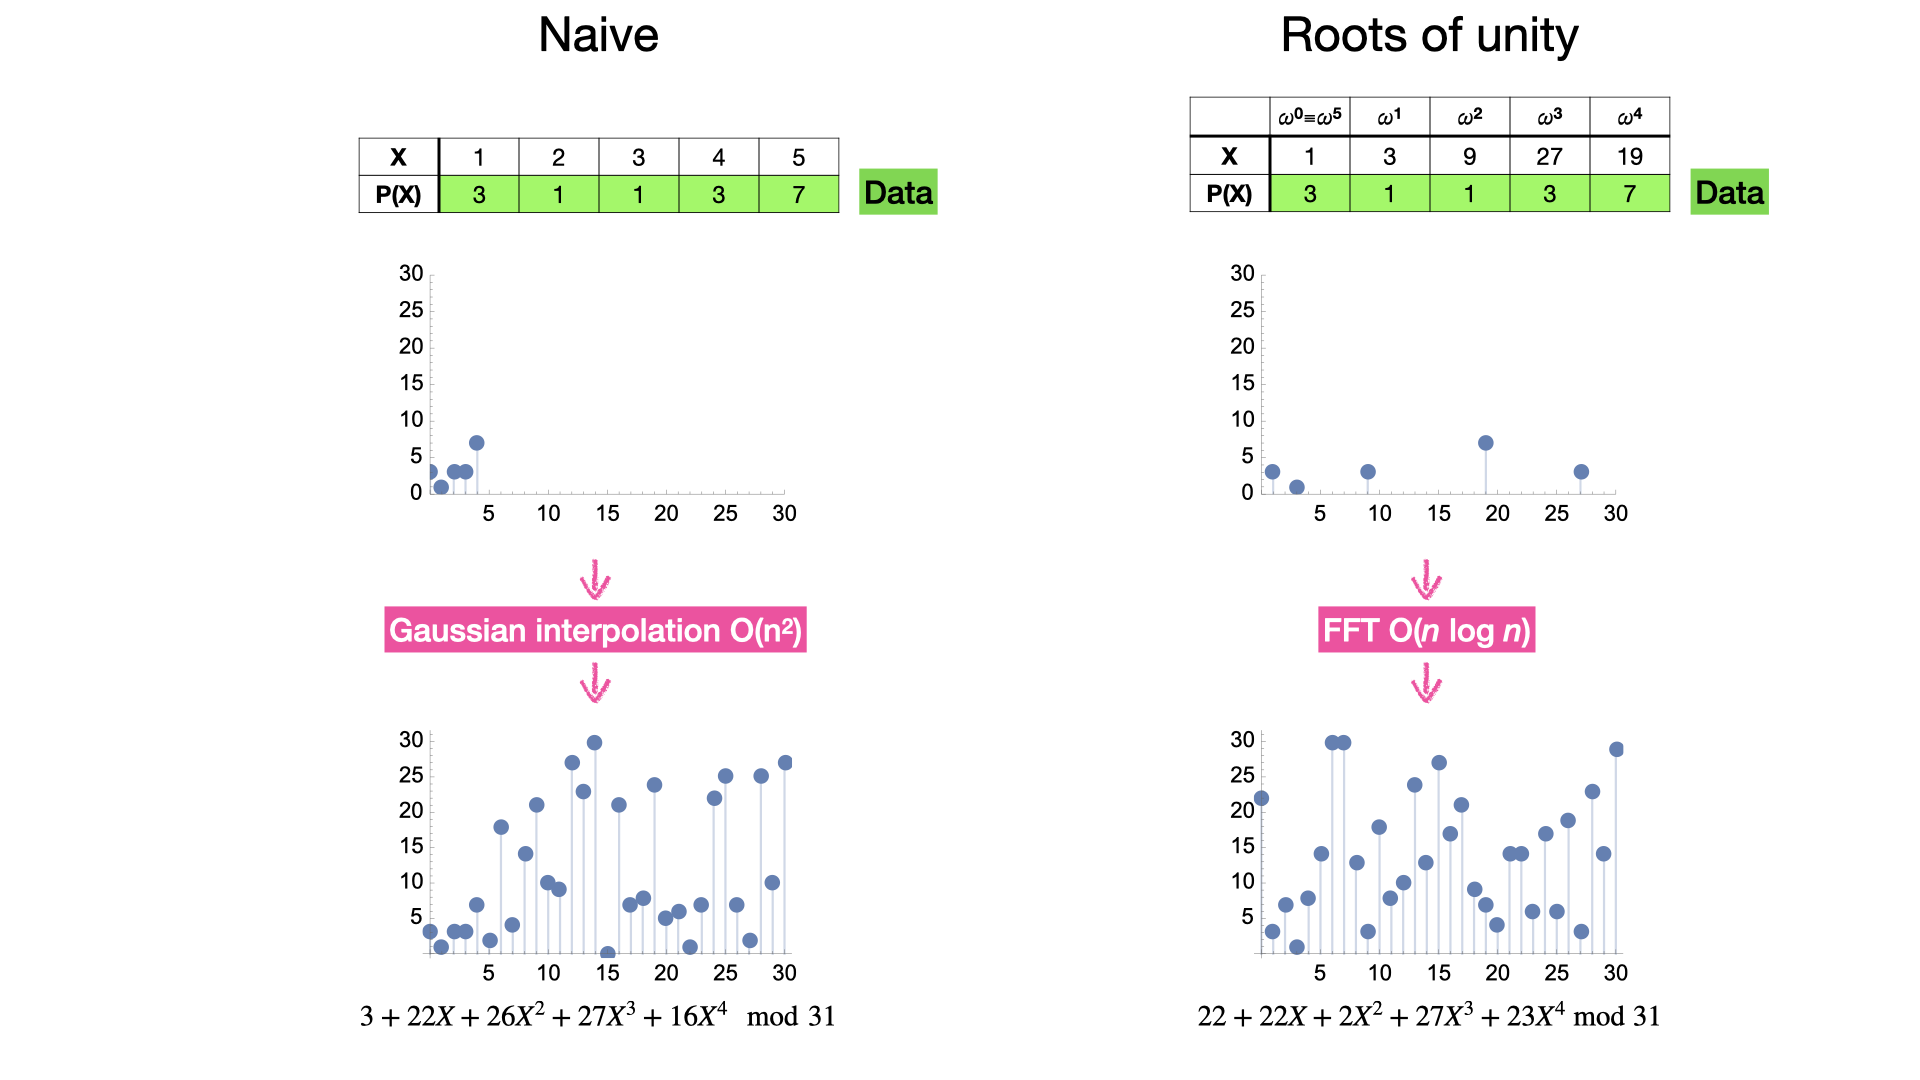
\includegraphics[width=\textwidth]{roots}
\caption{Small number ($\mathbb{Z}_{31}$) example of encoding a vector of integers $\tuple{3,1,1,3,7}$ into (a) the first 5 points of a polynomial, and (b) into 5th roots of unity ($\omega=3$).\label{fig:rou}}
\end{figure}

We use the approach of encoding data vectors into polynomials, committing to them using a polynomial commitment scheme (PCS), and forming zero knowledge arguments---a model called a polynomial-based interactive oracle proof (Poly-IOP). The zk-snark system Plonk popularized Poly-IOPs and has many extensions and optimizations. A one-dimensional vector of data is encoded into a univariate polynomial using 1 of 3 methods (all 3 are used at different steps of Plonk): (1) into the coefficients of the polynomial, (2) as roots of the polynomial, and (3) as the \(y\)-coordinates (\(\mathsf{data}_i=P(x_i)\)) of points on the polynomial. Plonk mostly relies on (3) and an interpolation algorithm is used to find the corresponding coefficients of the polynomial, which is
needed for the PCS. General interpolation algorithms are \(O(n^2)\) work for \(n\) evaluation points but this can be reduced to \(O(n\log n)\) with an optimization.

The optimization enables interpolation via the fast Fourier transform (FFT). It concerns how to choose the \(x\)-coordinates, which will serve as the index for accessing the data: evaluating \(P(X)\) at \(x_i\) will reveal \(\mathsf{data}_i\). First note, \(x\)-coordinates are from the exponent group (\(Z_q\)) and the choices exceed what is feasible to use (\(2^{255}\) values in \bls). Any subset can be used and interpolated. The optimization is to chose them with a mathematical structure. Specifically, instead an additive sequence (e.g., \(0,1,2,3,\ldots\)), we use a multiplicative sequence
\(1,\omega,\omega\cdot\omega,\omega\cdot\omega\cdot\omega,\ldots\) or equivalently: \(\omega^0,\omega^1,\omega^2,\ldots,\omega^{\kappa-1}\). Further, the sequence is closed under multiplication which means that next index after \(\omega^{\kappa-1}\) wraps back to the first index: \(\omega^{k-1} \cdot \omega = \omega^\kappa = \omega^0=1\) (this property is also useful in proving relationships between data in the vector and its neighbouring values).

For terminology, we say \(\omega\) is a generator with multiplicative order \(\kappa\) in \(Z_q\). This implies \(\omega^\kappa=1\). Rearranging, \(\omega=\sqrt[\kappa]{1}\). Thus we can equivalently describe \(\omega\) as a \(\kappa\)-th root of 1. Finally, as 1 is the unity element in \(Z_q\), \(\omega\) is commonly called a \(\kappa\)-th root of unity.

For practical purposes, \(\kappa\) represents the length of the longest vector of data we can use in our protocol. Where does \(\kappa\) come from? Different elements of \(Z_q\) will have different multiplicative orders but every order must be a divisor of \(q-1\). Thus \(\kappa\) is the largest divisor of the exact value of \(q\) used in an elliptic curve standard. The value of $q$ in \bls has \(\kappa=2^{32}\) (for terminology, this called a \(2\)-adicity of \(32\)).



